Churro extends the smooth-substitution problem introduced in \S\ref{sec:taxonomy}
beyond a single well-photographed page into a systematically fine-tuned model
evaluated across dozens of languages and scripts. Stanford OVAL's Churro 3B
\citep{semnani_churro_2025} is a continued-pretraining of
Qwen2.5-VL-3B-Instruct trained specifically to transcribe historical
documents; the \texttt{churro-dataset} test split on which we evaluate spans
29 language clusters and a comparable range of scripts, from Latin and
Cyrillic to Han, Devanagari, and Khmer. This combination makes Churro an
unusually direct testbed for two questions the taxonomy raises but cannot
answer from a single example: does training a model explicitly on
historical, multilingual transcription reduce fluent, plausible-but-unfaithful
readings, or does it simply relocate them; and is any such effect uniform, or
does it depend on how well a given language or script is represented in the
fine-tuning data? We compare Churro 3B against its own un-fine-tuned base
model, Qwen2.5-VL-3B-Instruct, on identical pages, so that every difference
we report below is attributable to Stanford's fine-tuning recipe specifically,
and not to a change in model architecture or scale.

We compute our semantic error score alongside CER and WER, the metrics
reported for Churro in the original paper \citep{semnani_churro_2025}, over
the same aligned ground-truth region so that both families of metrics
describe the same transcribed text. The two disagree more often than they
agree. Standard edit-distance metrics are, first, poorly behaved on several
of the scripts in the test set: because CER and WER are unbounded when a
prediction runs longer than its reference, character error rates exceed
1,000\% for Chinese, Japanese, Sanskrit, and Khmer, figures that describe a
numerical blow-up rather than a level of transcription quality. Second, and
more consequentially, low CER does not imply semantic fidelity: 318 pages in
our combined evaluation (13.6\%) have a CER under 10\% yet more than five
semantic errors each, split almost evenly between the base and fine-tuned
models. These are transcriptions a CER-only evaluation would certify as
successful while nonetheless containing the class of fluent, meaning-altering
substitution this paper is concerned with, and fine-tuning does not change the
rate at which this occurs---whatever Stanford's recipe optimizes for, it is
not the gap between surface accuracy and semantic faithfulness.

Considered on its own terms, Stanford's fine-tuning does reduce semantic
error substantially: averaged over all 29 languages, the semantic error rate
falls from 0.270 to 0.130 errors per ground-truth word
(Table~\ref{tab:churro-delta}), roughly a halving. But the average obscures
more than it reveals. The improvement ranges from a near-halving of semantic
error in Turkish and Persian to negligible effects in languages such as
English, and it is entangled with a second, less visible shift: the
fine-tuned model transcribes less of the page. Page coverage---the fraction
of the ground-truth text a model actually attempts---falls for 28 of the 29
languages under fine-tuning (Figure~\ref{fig:churro-coverage}), by as much as
49 points for Italian. Part of Churro's apparent gain in semantic fidelity is
therefore a gain in caution: transcribing a shorter, more confident span of
the page rather than the same span more faithfully. A fine-tuning result
reported as a single aggregate error rate can, in other words, be a coverage
effect in disguise.

Khmer is the one language in the test set where this pattern inverts, and it
is worth a brief note because the reversal is qualitative rather than
marginal. The base model does not produce Khmer script for these pages at
all; it hallucinates fluent, repeating Chinese text unrelated to the source,
consistent with Khmer's negligible presence in its pretraining data.
Churro's fine-tuning does teach the model to emit genuine Khmer script, but
on the same pages the fine-tuned model falls into a repetition loop,
generating a short Khmer phrase far past the length of the source page. The
result inflates edit-distance error and our semantic error count together,
and it inflates measured coverage as well, since a length-based coverage
heuristic cannot distinguish a longer correct transcription from a longer
degenerate one. Khmer therefore looks, in the aggregate tables, like
fine-tuning's single failure case; read against the actual output, it is
better described as a real capability gain---the model now attempts the
correct script---compromised by a decoding failure that our metrics,
semantic and traditional alike, register only as a much worse number.

\begin{figure}[h!]
  \centering
  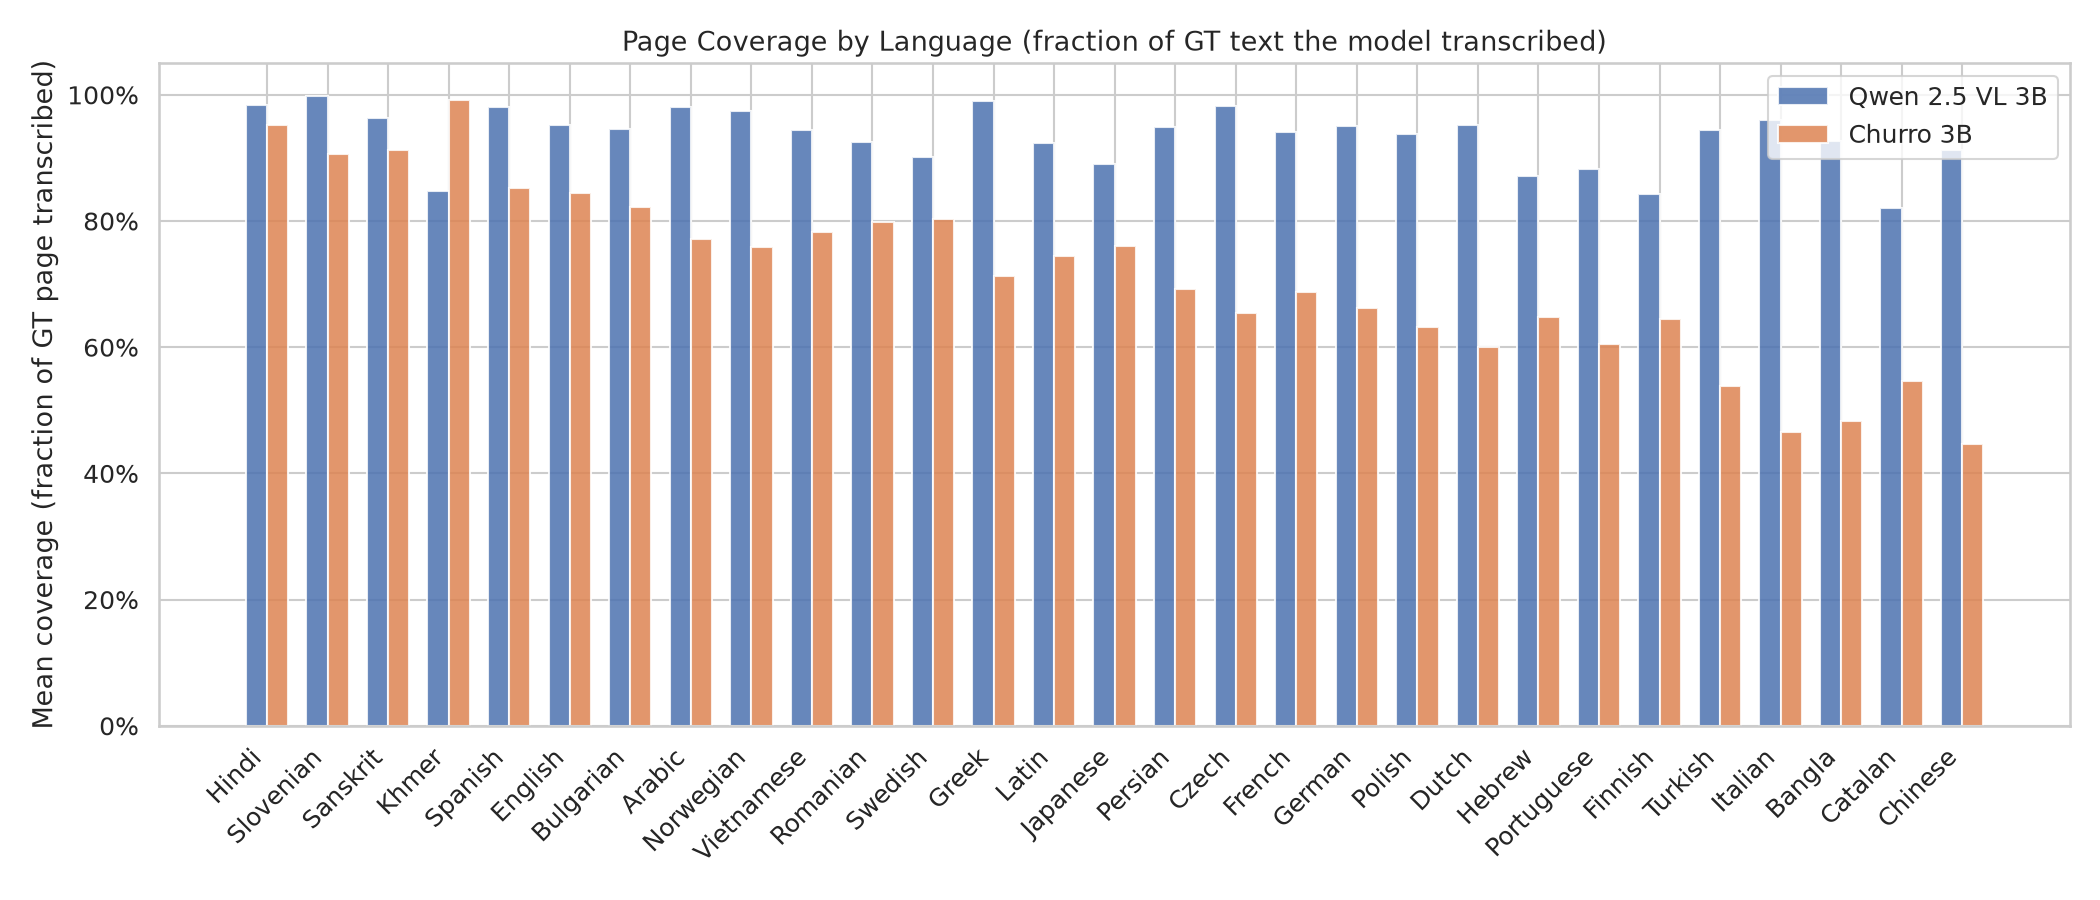
\includegraphics[width=\linewidth]{figures/01_coverage_by_language.png}
  \caption{Page coverage by language---the fraction of the ground-truth page
    each model transcribed. Stanford OVAL's fine-tuning lowers coverage for
    nearly every language; Khmer is the sole exception, for reasons discussed
    in the text.}
  \label{fig:churro-coverage}
\end{figure}

\begin{table}[h]
  \centering
  \caption{Semantic errors per ground-truth word, base model vs.\ Churro 3B,
    for representative languages. $\Delta = \text{Churro} - \text{Qwen}$;
    negative values indicate fine-tuning reduced semantic error. Full
    per-language results appear in the project repository.}
  \label{tab:churro-delta}
  \begin{tabular}{lrrr}
    \toprule
    Language & Qwen 2.5-VL-3B & Churro 3B & $\Delta$ \\
    \midrule
    Turkish  & 0.646 & 0.202 & $-0.444$ \\
    Persian  & 0.486 & 0.164 & $-0.322$ \\
    Greek    & 0.507 & 0.208 & $-0.299$ \\
    English  & 0.118 & 0.056 & $-0.062$ \\
    Khmer    & 0.133 & 0.708 & $+0.575$ \\
    \midrule
    \textbf{Mean (29 languages)} & \textbf{0.270} & \textbf{0.130} & \textbf{$-0.140$} \\
    \bottomrule
  \end{tabular}
\end{table}
